%        File: !comp!expand("%:p:t")!comp!
%     Created: !comp!strftime("%a %b %d %I:00 %p %Y ").substitute(strftime('%Z'), '\<\(\w\)\(\w*\)\>\(\W\|$\)', '\1', 'g')!comp!
% Last Change: !comp!strftime("%a %b %d %I:00 %p %Y ").substitute(strftime('%Z'), '\<\(\w\)\(\w*\)\>\(\W\|$\)', '\1', 'g')!comp!
%
\documentclass[a4paper]{article}
\usepackage[catalan]{babel}
\usepackage[utf8]{inputenc}
\usepackage[obeyspaces]{url}
\usepackage{comment}
\usepackage{hyperref}
\usepackage[pdftex]{graphicx}
\begin{document}
\title{Apunts sobre la tècnica de falcons}
\maketitle
\begin{abstract}
	Apunts sobre la tècnica de Falcons. Com pujar de pilar, com baixar, etc. O sigui, diferents postures i qüestions tècniques que moltes vegades s'assumeixen des de la colla com adquirides per els integrants que porten menys temps però que en canvi no \'es així. I lo pitjor de tot \'es que els nous no saben que no ho fan b\'e \ldots
\end{abstract}

\begin{comment}
oddsidemargin \the\oddsidemargin \newline
textwidth \the\textwidth \newline
marginparsep \the\marginparsep \newline
marginparwidth \the\marginparwidth \newline
hoffset \the\hoffset \newline
paperwidth \the\paperwidth 
\end{comment}

\section{La tècnica del pilar}
\paragraph{posició inicial \\}
Per pujar un pilar el primer que hem de fer \'es apropar-nos el màxim a la persona per on hem de pujar per no desesetabilitzar-la en la pujada. Ficarem el peu que està al terra (normalment l'esquerra) entre el mig de les cames de l'altre persona i l'altre peu el pujem el màxim que puguem, el qual farà despr\'es de palanca.

\scalebox{.5}{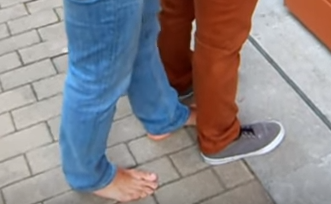
\includegraphics{pujar_inici.png}}
\paragraph{primer pas en la pujada \\}
El peu que està recolzat amb la cama de la persona per la qual es puja fa \textbf{força cap en fora i cap avall} de tal manera que el genoll i la cuixa fan força cap en dins i cap a dalt.
\paragraph{Segon pas. Pinzament}
En el següent pas el que hem de fer \'es pujar l'altra cama fins a l'altura de la que hem fet la palanca i pinzar la cadera de la persona per la que pujem. En aquesta posició, si la fem b\'e, ens hauríem de poder mantindre amb les mans lliures, de tal manera que puguem canviar la posició de les mans i posar-les en una postura que ens permetin fer força cap a munt amb elles.

\scalebox{.5}{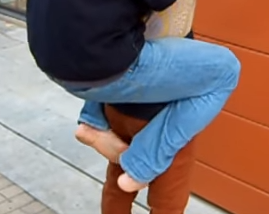
\includegraphics{pujar_pinzament.png}}
\paragraph{Últims pasos \\}
Mentre anem cap a munt busquem la faixa per a recolzar-hi el peu esquerra. Un cop allà, fem l'últim pas de la pujada i fiquem el genoll dret en l'espatlla del mateix costat de l'altre persona. Les mans dretes dels dos s'agafen, l'altra mà es recolza amb el cap del company i pujem el peu esquerra fins a quedar-nos d'empeus sobre ell, amb els peus ben a prop del coll per a que l'altre persona ens falqui amb les espatlles.

\scalebox{.5}{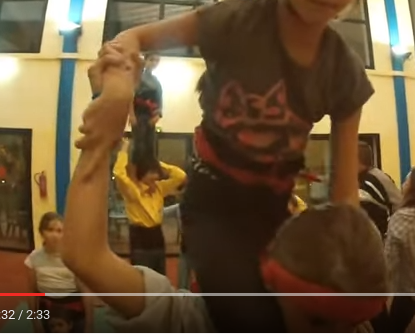
\includegraphics{genoll_espatlla.png}}
\paragraph{Baixar \\}
Per baixar, posem el genoll dret un altre cop sobre l'espatlla del company o la companya agafats de la mà dreta d'ella i amb l'altra peu busquem faixa. Un cop així rellisquem baixant posant els peus i cames en la postura de pinzament del segon pas de la pujada.

\scalebox{.5}{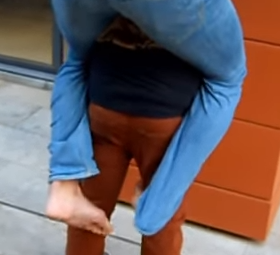
\includegraphics{baixar.png}}

\section{Sobre aquest document}
\textbf{Copyright}\copyright\ \textbf{\the\year\ Juan Aguilera}.\\
Permission is granted to copy, distribute and/or modify this document under the terms of the GNU Free Documentation License, Version 1.3 or any later version published by the Free Software Foundation;\\
with no Invariant Sections, no Front-Cover Texts, and no Back-Cover Texts.\\
A copy of the license is included in the section entitled \href{http://www.gnu.org/licenses/fdl.html}{``GNU Free Documentation License``}.

\begin{thebibliography}{99}
		% Exemple url: \bibitem{Debian} \url{https://wiki.debian.org/es}%
	\bibitem{PUJAR_I} \url{https://www.youtube.com/watch?v=HmezLTOYjts}
	\bibitem{PUJAR_II} \url{https://www.youtube.com/watch?v=SSgmBMufVXw}
\end{thebibliography}

\end{document}


